%======================================================================
\chapter{Algorithms Used}
%======================================================================

\section{A Segmentation Problem}
Image segmentation is a process of dividing a digital image into multiple segments or regions, each of which corresponds to a distinct object or part of the image. The goal of image segmentation is to simplify the image representation by partitioning it into meaningful regions, which can then be used for analysis, manipulation, or understanding.

There are several methods for image segmentation, including thresholding, edge detection, region growing, clustering, and machine learning-based methods. Thresholding is a simple method that segments an image by setting a threshold value and classifying pixels based on whether they are above or below the threshold. Edge detection methods identify boundaries between regions by detecting sharp changes in image intensity. Region growing methods start from a seed point and iteratively add neighboring pixels that meet certain criteria. Clustering methods group pixels based on their similarity in feature space. Machine learning-based methods use algorithms such as decision trees, random forests, and deep neural networks to learn the mapping between image features and segment labels

\section{DataSet}
Segmented Labels are available in \cite{five}
The LandCover.ai (Land Cover from Aerial Imagery) dataset is a dataset for automatic mapping of buildings, woodlands, water and roads from aerial images.
\subsection{Dataset Features}
\begin{enumerate}
    \item land cover from Poland, Central Europe 
    \item three spectral bands - RGB
    \item 33 orthophotos with 25 cm per pixel resolution (~9000x9500 px)
    \item 8 orthophotos with 50 cm per pixel resolution (~4200x4700 px)
    \item total area of 216.27 km2
\end{enumerate}
\subsection{Labels}
\begin{enumerate}
    \item classes: building (1), woodland (2), water(3), road(4)
    \item areas: 1.85 km2 of buildings, 72.02 km2 of woodlands, 13.15 km2 of water, 3.5 km2 of roads
\end{enumerate}

\section{UNet Architecture}
The U-Net architecture is a type of neural network that is commonly used for image segmentation tasks. It was specifically designed for biomedical image segmentation, but has also been used for other types of image segmentation.

What makes the U-Net architecture unique is its use of a contracting path and an expansive path. The contracting path is a series of convolutional and pooling layers that reduce the spatial resolution of the image, while also increasing the number of feature channels. This helps the network learn high-level features from the input image.

The expansive path is a series of upsampling and convolutional layers that increase the spatial resolution of the image, while reducing the number of feature channels. This helps the network create a segmentation map that has the same spatial resolution as the input image.


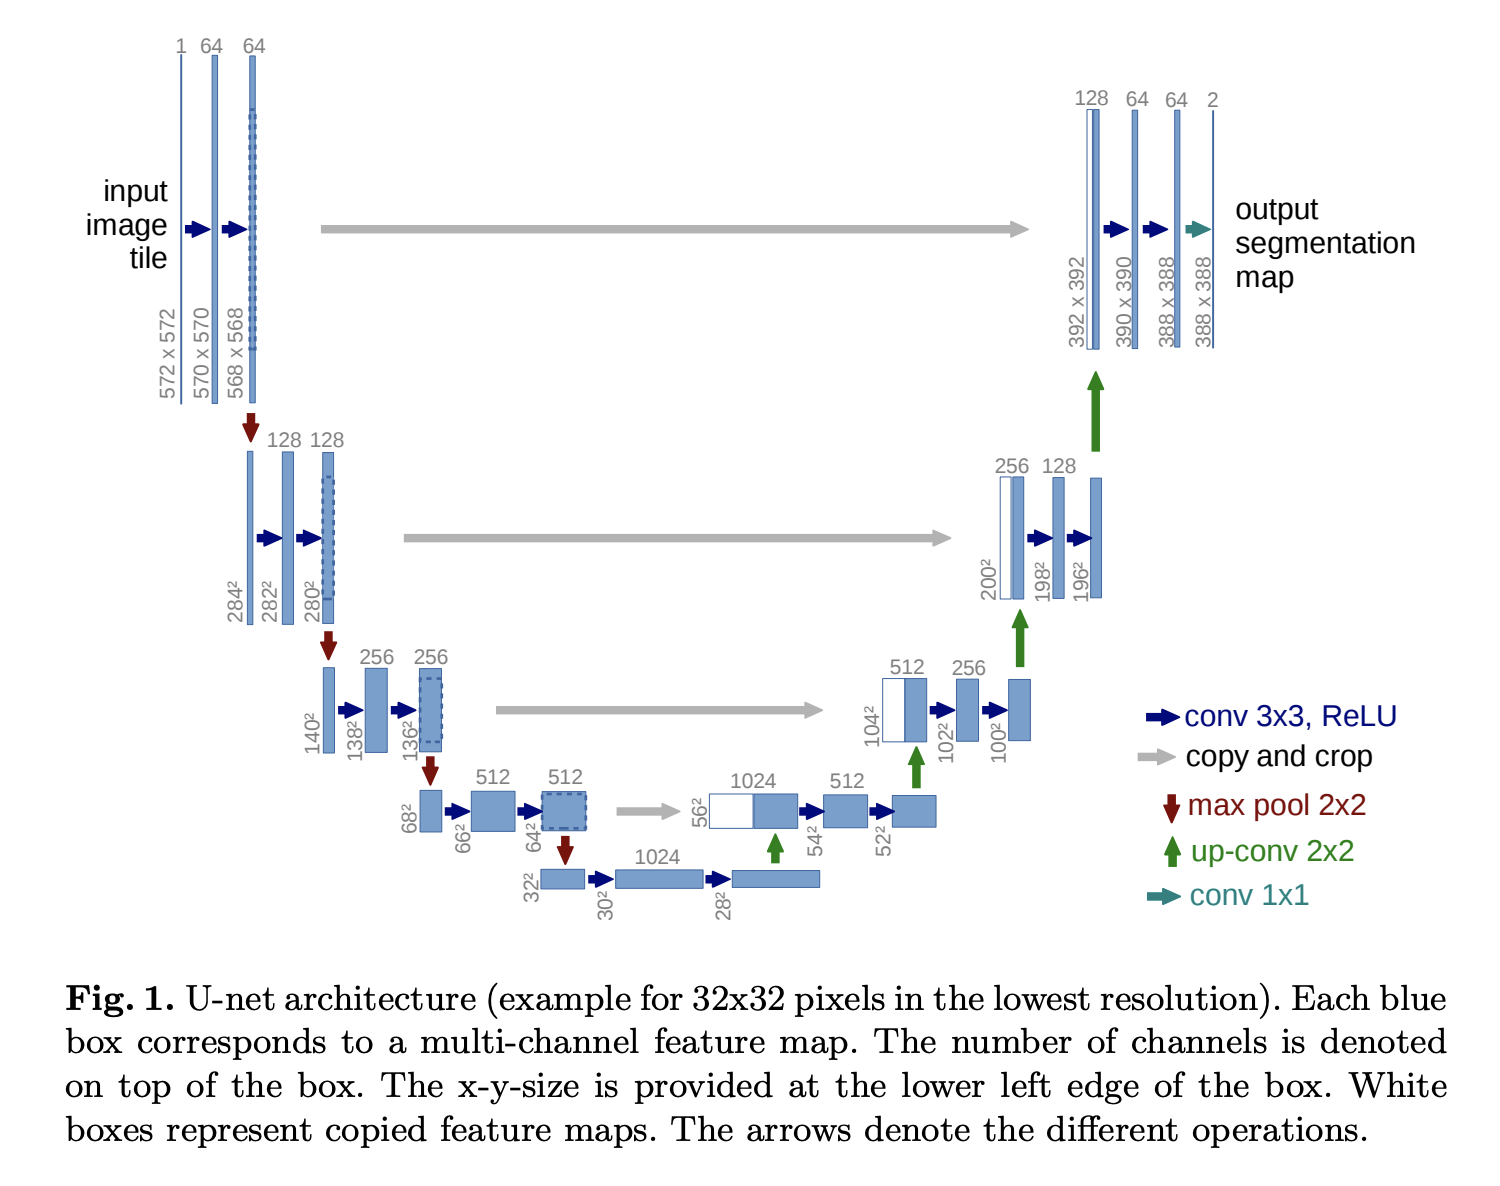
\includegraphics[scale=0.6]{images/1.png}
\subsection{Usecases of UNet Architecture}
The U-Net architecture is particularly useful for segmentation problems because it can effectively capture both local and global features. The encoder network can capture global features such as context and image-level information, while the decoder network can capture local features such as object boundaries and fine details. The skip connections help propagate information across the network, improving the accuracy of the segmentation. Additionally, the U-Net architecture is computationally efficient and can be trained on relatively small datasets, making it a practical choice for various segmentation tasks.
\begin{enumerate}
    \item High Accuracy: The U-Net model has shown to achieve high accuracy in various image segmentation tasks, including medical image segmentation and object detection in satellite imagery.
    \item Efficient use of data: The architecture makes efficient use of the available training data by utilizing the skip connections. The skip connections allow the network to combine low-level and high-level features, which helps in reducing the problem of vanishing gradients.
    \item Reduced Overfitting: The architecture uses data augmentation techniques, such as flipping, rotating, and zooming, which helps in preventing overfitting.
    \item Fast and Easy Training: The architecture is relatively easy to train, and training times are faster compared to other complex architectures.
\end{enumerate}

